\section{∞-\trCategories{}的\trYoneda{}引理}
\label{sec:yoneda-lemma}

在本节中，我们将证明\trYoneda{}引理的∞-范畴版本。利用我们在 3.3 节中讨论过的%
\trStraightening{}--\trUnstraightening{}\trEquivalence{}，我们借助%
\trTwistedArrowCategory{}，循\trLurie{}在 \cite{Lur17} 中的构造，来构造一个\trBivariant{}%
\trMappingSpace{}\trFunctor{} $\C^{\mathrm{op}} \times \C \to \mathrm{Spc}$。随后，我们将以%
\trLeftFibration{}的语言陈述并概述\trYoneda{}引理的一个证明。此外，我们将指出如何
由这条引理推出：与\trBivariant{}\trMappingSpace{}\trFunctor{}相关联的\trFunctor{}%
$\C \to \mathrm{Fun}(\C^{\mathrm{op}}, \mathrm{Spc})$ 是\trFullyFaithful{}——
这正是该\trFunctor{}得名\emph{\trYoneda{}嵌入}（Yoneda embedding）的缘由。

首先，我们希望证明：对每个∞-\trCategory{} $\C$，都存在一个\trYoneda{}\trFunctor{}%
$\C \to \mathrm{Fun}(\C^{\mathrm{op}}, \mathrm{Spc})$，它应当把 $\C$ 的一个%
\trObject{} $x$ 送到\trFunctor{} $y \mapsto \mathrm{map}_{\C}(y, x)$。随后，我们将
指出这个\trFunctor{}是\trFullyFaithful{}，这便是\trYoneda{}引理的∞-范畴版本。至于
$\mathrm{map}_{\C}(-, x)$ 对每个单独的 $x$ 而言是一个\trFunctor{}，这已是我们已知的事情。

\begin{definition}\label{def:map-functor}
设 $x$ 是∞-\trCategory{} $\C$ 的一个\trObject{}。那么\trFunctor{} $\C_{/x} \to \C$
是一个\trRightFibration{}，从而，由第 3 章中的\cref{thm:lfib-straightening}
（应用于 $\C^{\mathrm{op}}$），它等价地由一个\trFunctor{}%
$\C^{\mathrm{op}} \to \mathrm{Spc}$ 给出，后者把 $y$ 送到
$\C_{/x} \times_{\C} \{y\} \simeq \mathrm{map}_{\C}(y, x)$。我们将把这个\trFunctor{}记作
$\mathrm{map}_{\C}(-, x)$。
\end{definition}

我们现在的任务是说明：诸\trFunctor{} $\mathrm{map}_{\C}(-, x)$ 在 $x$ 上是\trFunctor{}性的。
我们从一个构造开始。

\begin{lemma}\label{lem:join-cosimplicial}
对应关系 $[n] \mapsto [n] \star [n]^{\mathrm{op}} \cong [2n+1]$ 可扩充为一个%
\trFunctor{} $\Delta \to \Delta$。特别地，把 $[n]$ 送到
$\Delta^n \star (\Delta^n)^{\mathrm{op}}$ 便给出\trSimplicialSets{}中一个%
\trCosimplicial{}对象，即一个\trFunctor{} $\Delta \to \mathrm{sSet}$。
\end{lemma}

\begin{definition}\label{def:twisted-arrow}
设 $\C$ 是一个∞-\trCategory{}。我们将其\emph{\trTwistedArrowCategory{}}（twisted
arrow category）$\mathrm{Tw}(\C)$ 定义为\trSimplicialSet{}%
\[
\mathrm{Tw}(\C)_n
  = \mathrm{Hom}_{\mathrm{sSet}}\bigl(\Delta^n \star (\Delta^n)^{\mathrm{op}}, \C\bigr),
\]
其单纯结构来自\trCosimplicial{}对象
$[n] \mapsto \Delta^n \star (\Delta^n)^{\mathrm{op}}$。包含映射
$\Delta^n \to \Delta^n \star (\Delta^n)^{\mathrm{op}} \leftarrow (\Delta^n)^{\mathrm{op}}$
确定出一个\trFunctor{}%
\[
\mathrm{Tw}(\C) \longrightarrow \C \times \C^{\mathrm{op}}.
\]
\end{definition}

下述命题的证明取自 \cite{Lur17} 中的命题 5.2.1.3。

\begin{proposition}\label{prop:twisted-arrow-right-fibration}
对∞-\trCategory{} $\C$ 而言，\trFunctor{}%
\[
\mathrm{Tw}(\C) \longrightarrow \C \times \C^{\mathrm{op}}
\]
是一个\trRightFibration{}。特别地，$\mathrm{Tw}(\C)$ 仍是一个∞-\trCategory{}。
\end{proposition}

\begin{proof}
设 $0 < k \le n$，并考虑\trLiftingProblem{}%
\begin{center}
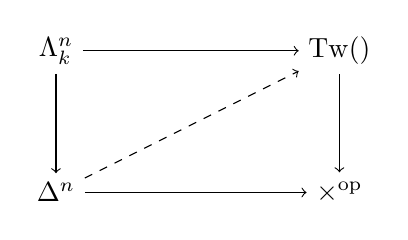
\begin{tikzpicture}
  \node (lk) at (0,0) {$\Lambda^n_k$};
  \node (tw) at (3.6,0) {$\mathrm{Tw}(\C)$};
  \node (dn) at (0,-1.8) {$\Delta^n$};
  \node (cp) at (3.6,-1.8) {$\C \times \C^{\mathrm{op}}$};
  \draw[->] (lk) -- (tw);
  \draw[->] (lk) -- (dn);
  \draw[->] (tw) -- (cp);
  \draw[->] (dn) -- (cp);
  \draw[->, dashed] (dn) -- (tw);
\end{tikzpicture}
\end{center}
把\trTwistedArrowCategory{}的定义展开，这相当于\trLiftingProblem{}%
\begin{center}
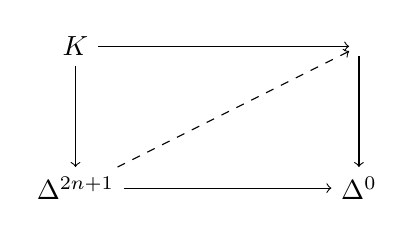
\begin{tikzpicture}
  \node (k) at (0,0) {$K$};
  \node (c) at (3.6,0) {$\C$};
  \node (dn) at (0,-1.8) {$\Delta^{2n+1}$};
  \node (d0) at (3.6,-1.8) {$\Delta^0$};
  \draw[->] (k) -- (c);
  \draw[->] (k) -- (dn);
  \draw[->] (c) -- (d0);
  \draw[->] (dn) -- (d0);
  \draw[->, dashed] (dn) -- (c);
\end{tikzpicture}
\end{center}
其中 $K$ 是 $\Delta^{2n+1}$ 的一个子单纯集，由满足下述三条性质之一的那些面
$\sigma$ 组成：
\begin{enumerate}[label=(\arabic*)]
  \item $\sigma$ 含于
        $\Delta^{\langle 0, \dots, n\rangle} \subseteq \Delta^{2n+1}$ 之中。
  \item $\sigma$ 含于
        $\Delta^{\langle n+1, \dots, 2n+1\rangle} \subseteq \Delta^{2n+1}$ 之中。
  \item 存在 $j \ne k$，$0 \le j \le n$，使得 $j$ 与 $2n+1-j$ 都不是 $\sigma$
        的顶点。
\end{enumerate}
由于 $\C$ 是∞-\trCategory{}，只需证明包含映射 $K \to \Delta^{2n+1}$ 是%
\trInnerAnodyne{}的。我们称一个\trSimplex{} $\sigma$ 是\emph{主的}（primary），如果它不含于
$K$，且其顶点都含于集合 $\{k, \dots, 2n+1\}$ 之中；相应地，若 $\sigma$ 不含于 $K$
且不是主的，我们便称它为\emph{次的}（secondary）。我们令 $S$ 为由 $\Delta^{2n+1}$
的下述\trSimplex{} $\tau$ 组成的集合：
\begin{enumerate}[label=(\arabic*)]
  \item $\tau$ 是主的，且 $k$ 不是 $\tau$ 的顶点；
  \item $\tau$ 是次的，且 $2n+1-k$ 不是 $\tau$ 的顶点。
\end{enumerate}
给定 $S$ 中的一个\trSimplex{} $\tau$，我们令 $\tau'$ 为下述方式得到的\trSimplex{}：若 $\tau$ 是主的，
则添加顶点 $k$；若 $\tau$ 是次的，则添加 $2n+1-k$。我们观察到，$\Delta^{2n+1}$ 的
每个\trSimplex{}要么含于 $K$，要么含于 $S$，要么形如 $\tau'$，其中 $\tau \in S$ 唯一：倘若它
既不含于 $K$ 也不含于 $S$，那么它要么是主的且以 $k$ 为顶点，要么是次的且以
$2n+1-k$ 为顶点；无论哪种情形，都可以删去顶点 $k$ 或 $2n+1-k$，从而按需要得到
一个主的或次的\trSimplex{}。

我们现在选取 $S$ 的一个排序 $\{\sigma_1, \sigma_2, \dots, \sigma_m\}$，使之具有
下述两条性质：
\begin{enumerate}[label=(\arabic*)]
  \item 若 $p \le q$，则 $\dim(\sigma_p) \le \dim(\sigma_q)$。
  \item 若 $p \le q$，$\dim(\sigma_p) = \dim(\sigma_q)$，且 $\sigma_q$ 是主的，
        那么 $\sigma_p$ 也是主的。
\end{enumerate}
对 $0 \le q \le m$，我们令 $K_q$ 为从 $K$ 出发添加诸\trSimplex{} $\sigma_p$ 与
$\sigma'_p$（$1 \le p \le q$）所得的 $\Delta^{2n+1}$ 的子单纯集。显然，
$K_m = \Delta^{2n+1}$，于是我们得到一个\trFiltration{}%
\[
K \to K_1 \to K_2 \to \cdots \to K_m = \Delta^{2n+1},
\]
且只需证明：对每个 $q$，映射 $K_{q-1} \to K_q$ 是\trInnerAnodyne{}的。由于 $K_q$
是从 $K_{q-1}$ 添加\trSimplex{} $\sigma_q$ 与 $\sigma'_q$ 得到的，而 $\sigma'_q$ 包含
$\sigma_q$，故只需证明存在一个\trPushout{}图表
\begin{center}
\begin{tikzpicture}
  \node (lj) at (0,0) {$\Lambda^d_j$};
  \node (kq1) at (3.6,0) {$K_{q-1}$};
  \node (dd) at (0,-1.8) {$\Delta^d$};
  \node (kq) at (3.6,-1.8) {$K_q$};
  \draw[->] (lj) -- (kq1);
  \draw[->] (lj) -- (dd);
  \draw[->] (kq1) -- (kq);
  \draw[->] (dd) -- node[above] {$\sigma'_q$} (kq);
\end{tikzpicture}
\end{center}
其中 $d$ 是 $\sigma'_q$ 的维数，且 $0 < j < d$。为此，我们需要查明 $\sigma'_q$
的诸面中哪些已含于 $K_{q-1}$，并论证恰好有一个\trInnerFace{}不含于 $K_{q-1}$。
\end{proof}

\begin{definition}\label{def:map-bivariant}
对每个∞-\trCategory{}，我们把与\trRightFibration{}%
$\mathrm{Tw}(\C) \to \C \times \C^{\mathrm{op}}$ 相关联的\trFunctor{}记作
$\mathrm{map}_{\C}(-, -)\colon \C^{\mathrm{op}} \times \C \to \mathrm{Spc}$。
\end{definition}

\begin{remark}\label{rem:alternative-mapping-functor}
我们本可以走另一条路：如果只想构造映射\trFunctor{}%
$\mathrm{map}_{\C}(-, -)\colon \C^{\mathrm{op}} \times \C \to \mathrm{Spc}$，
那么可以观察到，按定义 $\mathrm{Spc} = \mathrm{N}(\mathrm{Kan})$。因此，这样的%
\trFunctor{}等价地由一个单纯\trFunctor{}%
$\mathfrak{C}[\C^{\mathrm{op}} \times \C] \to \mathrm{Kan}$
给出。于是我们可以考虑复合
\[
\mathfrak{C}[\C^{\mathrm{op}} \times \C]
  \to \mathfrak{C}[\C]^{\mathrm{op}} \times \mathfrak{C}[\C]
  \to \mathrm{Kan},
\]
其中第一部分由典范映射给出，第二部分则由单纯\trMappingSpace{}再接一个\trFunctor{}性的
Kan-替换给出。这一版本的\trBivariant{}\trMappingSpace{}\trFunctor{}（至少逐点地）等价于我们的做法，
其确认由 \cite{Lur09} 中的定理 1.1.5.13 给出。
\end{remark}

\begin{lemma}\label{lem:slice-twisted-fibre}
设 $\C$ 是一个∞-\trCategory{}，$x$ 是 $\C$ 的一个\trObject{}。那么存在一个交换图表
\begin{center}
\begin{tikzpicture}
  \node (cx) at (0,0) {$\C_{/x}$};
  \node (tw) at (4.2,0) {$\mathrm{Tw}(\C)$};
  \node (cpx) at (0,-2.0) {$\C \times \{x\}$};
  \node (cp) at (4.2,-2.0) {$\C \times \C^{\mathrm{op}}$};
  \draw[->] (cx) -- (tw);
  \draw[->] (cx) -- (cpx);
  \draw[->] (tw) -- (cp);
  \draw[->] (cpx) -- (cp);
\end{tikzpicture}
\end{center}
该图表是\trHomotopyCartesian{}。换言之，诱导映射
$\C_{/x} \to \mathrm{Tw}(\C)_x$ 是 $\C$ 之上的诸\trRightFibration{}之间的一个%
\trJoyalEquivalence{}。
\end{lemma}

\begin{proof}
我们回忆：$\mathrm{Tw}(\C)_x$ 的 $n$-\trSimplex{}由那些映射
$\Delta^n \star (\Delta^n)^{\mathrm{op}} \to \C$ 给出，它们沿包含映射
$(\Delta^n)^{\mathrm{op}} \to \Delta^n \star (\Delta^n)^{\mathrm{op}}$ 的限制
恰为在 $\C$ 的\trObject{} $x$ 处取常值的那个映射。然后我们定义一个辅助的%
\trSimplicialSet{} $\mathcal{M}$，其 $n$-\trSimplex{}由那些映射
$\Delta^n \star \Delta^0 \star (\Delta^n)^{\mathrm{op}} \to \C$ 给出，它们沿
$\varnothing \star \Delta^0 \star (\Delta^n)^{\mathrm{op}} \to \Delta^n \star \Delta^0 \star (\Delta^n)^{\mathrm{op}}$
的限制在 $x$ 处取常值。
诸显然的包含映射定义出映射
\[
\C_{/x} \leftarrow \mathcal{M} \to \mathrm{Tw}(\C)_x,
\]
且左边的映射容有一个\trSectionMap{}，它由映射
$\Delta^0 \star (\Delta^n)^{\mathrm{op}} \to \Delta^0$ 诱导而来。于是只需证明
上述两个映射都是\trJoyalEquivalence{}。这通过证明两个映射都是%
\trTrivialFibration{}来完成，也就是说，它们对诸\trBoundaryInclusion{}满足提升
性质。让我们从 $\mathcal{M} \to \C_{/x}$ 的情形开始，考虑\trLiftingProblem{}%
\begin{center}
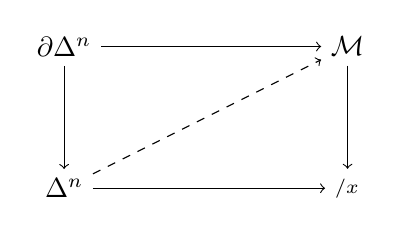
\begin{tikzpicture}
  \node (bd) at (0,0) {$\partial\Delta^n$};
  \node (m) at (3.6,0) {$\mathcal{M}$};
  \node (dn) at (0,-1.8) {$\Delta^n$};
  \node (cx) at (3.6,-1.8) {$\C_{/x}$};
  \draw[->] (bd) -- (m);
  \draw[->] (bd) -- (dn);
  \draw[->] (m) -- (cx);
  \draw[->] (dn) -- (cx);
  \draw[->, dashed] (dn) -- (m);
\end{tikzpicture}
\end{center}
把诸定义展开可见，这等价地由一个\trLiftingProblem{}给出
\begin{center}
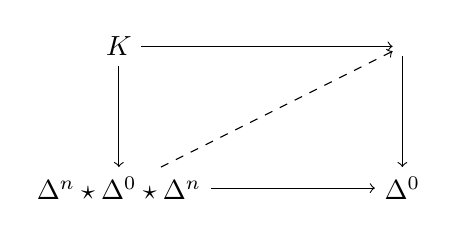
\begin{tikzpicture}
  \node (k) at (0,0) {$K$};
  \node (c) at (3.6,0) {$\C$};
  \node (dn) at (0,-1.8) {$\Delta^n \star \Delta^0 \star \Delta^n$};
  \node (d0) at (3.6,-1.8) {$\Delta^0$};
  \draw[->] (k) -- (c);
  \draw[->] (k) -- (dn);
  \draw[->] (c) -- (d0);
  \draw[->] (dn) -- (d0);
  \draw[->, dashed] (dn) -- (c);
\end{tikzpicture}
\end{center}
其中 $K$ 表示包含
$\Delta^n \star \Delta^0 \star \varnothing$、
$\varnothing \star \Delta^0 \star \Delta^n$ 以及
$\Delta^I \star \Delta^0 \star (\Delta^I)^{\mathrm{op}}$（对每个真子集
$I \subseteq [n]$）的最小子单纯集。由第 2 章中的%
\cref{thm:isofibration-lifting-joyal-equivalence}，只需证明包含映射
$K \to \Delta^n \star \Delta^0 \star \Delta^n$ 是一个\trJoyalEquivalence{}。
首先，我们断言：复合
\[
\Delta^n \star \Delta^0 \amalg_{\Delta^0} \Delta^0 \star \Delta^n
  \to K \to \Delta^n \star \Delta^0 \star \Delta^n
\]
是一个\trJoyalEquivalence{}。为看出这一点，我们考虑图表
\begin{center}
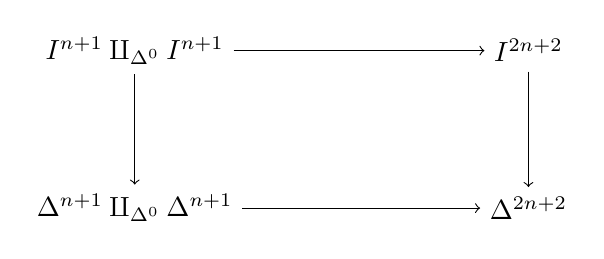
\begin{tikzpicture}
  \node (ia) at (0,0) {$I^{n+1} \amalg_{\Delta^0} I^{n+1}$};
  \node (ib) at (5.0,0) {$I^{2n+2}$};
  \node (da) at (0,-2.0) {$\Delta^{n+1} \amalg_{\Delta^0} \Delta^{n+1}$};
  \node (db) at (5.0,-2.0) {$\Delta^{2n+2}$};
  \draw[->] (ia) -- (ib);
  \draw[->] (ia) -- (da);
  \draw[->] (ib) -- (db);
  \draw[->] (da) -- (db);
\end{tikzpicture}
\end{center}
其中上方的水平映射是一个同构，而下方的水平映射是正在研究中的那个映射。于是只需
证明两个竖直映射都是\trJoyalEquivalence{}。对右边这个，这由如下事实得出：\trSpineInclusion{}%
是\trInnerAnodyne{}的（第 1 章中的\cref{prop:spine-inner-anodyne}），从而是一个%
\trJoyalEquivalence{}（第 2 章中的\cref{cor:inner-anodyne-joyal-equivalence}）。
对左边的竖直映射，我们对诸映射 $I^{n+1} \to \Delta^{n+1}$ 作同样的论证，然后用
第 2 章中的\cref{cor:pushout-joyal-equivalence}得出：\trPushout{}上的映射也是%
\trJoyalEquivalence{}。现在只需证明映射
\[
\Delta^n \star \Delta^0 \amalg_{\Delta^0} \Delta^0 \star \Delta^n \to K
\]
是一个\trJoyalEquivalence{}。我们把 $K$ 中由形如
$\Delta^I \star \Delta^0 \star (\Delta^I)^{\mathrm{op}}$（其中
$I \subseteq [n]$ 是真子集）的\trSimplex{}张成的子单纯集记作 $K_0$。由于图表
\begin{center}
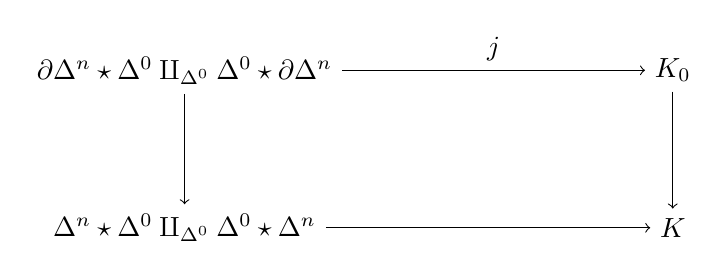
\begin{tikzpicture}
  \node (bd) at (0,0)
    {$\partial\Delta^n \star \Delta^0 \amalg_{\Delta^0} \Delta^0 \star \partial\Delta^n$};
  \node (k0) at (6.2,0) {$K_0$};
  \node (dn) at (0,-2.0)
    {$\Delta^n \star \Delta^0 \amalg_{\Delta^0} \Delta^0 \star \Delta^n$};
  \node (k) at (6.2,-2.0) {$K$};
  \draw[->] (bd) -- node[above] {$j$} (k0);
  \draw[->] (bd) -- (dn);
  \draw[->] (k0) -- (k);
  \draw[->] (dn) -- (k);
\end{tikzpicture}
\end{center}
是一个\trPushout{}图表，只需证明映射 $j$ 是一个\trJoyalEquivalence{}。但这个映射是形如
\[
\Delta^I \star \Delta^0 \amalg_{\Delta^0} \Delta^0 \star (\Delta^I)^{\mathrm{op}}
  \to \Delta^I \star \Delta^0 \star (\Delta^I)^{\mathrm{op}}
\]
的映射的\trColimit{}，而这些映射恰是我们刚才论证过其为\trJoyalEquivalence{}的那些。于是
我们得出结论：映射 $\mathcal{M} \to \C_{/x}$ 是一个\trJoyalEquivalence{}。

尚待证明的是，映射 $\mathcal{M} \to \mathrm{Tw}(\C)_x$ 也是一个%
\trJoyalEquivalence{}。由于该证明在精神上与\cref{prop:twisted-arrow-right-fibration}
的证明十分相似，我们将不再详述其细节，而是转而参考 \cite{Lur17} 中的命题
5.2.1.10。
\end{proof}

\begin{corollary}\label{cor:fibre-composite-map}
对每个\trObject{} $x$，复合
$\C \times \{x\} \to \C \times \C^{\mathrm{op}} \to \mathrm{Spc}$
等价于\trFunctor{} $\mathrm{map}_{\C}(-, x)$。
\end{corollary}

\begin{proof}
第一个\trFunctor{}是与\trRightFibration{} $\mathrm{Tw}(\C)_x \to \C$ 相关联的那个\trFunctor{}，
而另一个\trFunctor{}则与\trRightFibration{} $\C_{/x} \to \C$ 相关联。由%
\cref{lem:slice-twisted-fibre}与第 2 章中的\cref{prop:slice-fat-slice-joyal-equivalence}，
这两个\trRightFibration{}是等价的。于是，断言由\trStraightening{}--%
\trUnstraightening{}\trEquivalence{}（第 3 章中的\cref{thm:lfib-straightening}）得出。
\end{proof}

\begin{definition}\label{def:yoneda-functor}
设 $\C$ 是一个∞-\trCategory{}。\trFunctor{}%
$\mathrm{map}_{\C}(-, -)\colon \C^{\mathrm{op}} \times \C \to \mathrm{Spc}$
\trAdjunction{}于一个\trFunctor{}%
$Y\colon \C \to \mathrm{Fun}(\C^{\mathrm{op}}, \mathrm{Spc})$，我们把这个\trFunctor{}称为%
\emph{\trYoneda{}\trFunctor{}}（Yoneda functor）。
\end{definition}

下述结果就是\trYoneda{}引理的∞-范畴版本。

\begin{proposition}\label{prop:yoneda-lemma}
设 $F\colon \C \to \mathrm{Spc}$ 是一个\trFunctor{}，并设 $x$ 是 $\C$ 的一个%
\trObject{}。那么，由在恒同处求值给出的典范映射
\[
\mathrm{map}_{\mathrm{Fun}(\C, \mathrm{Spc})}(\mathrm{map}_{\C}(x, -), F) \to F(x)
\]
是一个\trEquivalence{}。
\end{proposition}

\begin{proof}
我们设 $p\colon \E \to \C$ 为对应于\trFunctor{} $F$ 的那个\trLeftFibration{}。在来自第 3 章中的%
\cref{thm:lfib-straightening}的\trStraightening{}--\trUnstraightening{}\trEquivalence{}之下，
\[
\mathrm{Fun}(\C, \mathrm{Spc}) \simeq
  \mathrm{LFib}(\C) \overset{\mathrm{full}}{\subseteq} \mathrm{Cat}_{\infty}/\C,
\]
左边的诸\trMappingSpace{}对应于
$\mathrm{map}_{\mathrm{Cat}_{\infty}/\C}(\C_{x/}, \E)$。我们断言：存在一个典范\trEquivalence{}%
\[
\mathrm{map}_{\mathrm{Cat}_{\infty}/\C}(\C_{x/}, \E) \simeq
  \mathrm{Fun}_q(\C_{x/}, \E),
\]
其中 $q\colon \C_{x/} \to \C$ 是典范的\trForgetfulFunctor{}，而
$\mathrm{Fun}_q(\C_{x/}, \E)$ 与第 3 章中的\cref{def:fun-mcc}中的一样，只是不带
那些上标。

暂时姑且承认这一点，我们需要证明映射
\[
\mathrm{Fun}_q(\C_{x/}, \E) \to
  \mathrm{Fun}_{\mathrm{id}_x}(\Delta^0, \E) \cong \E_x
\]
是一个等价。为此，回忆一下：由\trStraightening{}--\trUnstraightening{}\trEquivalence{}的
构造，存在一个典范\trEquivalence{} $\E_x \simeq F(x)$。这里，该映射由指明 $x$ 的恒同的典范映射
$\Delta^0 \to \C_{x/}$ 诱导。由\cref{ex:terminal-object-slice}，$x$ 的恒同是 $\C_{x/}$ 的一个%
\trInitialObject{}，从而映射 $\Delta^0 \to \C_{x/}$ 是\trLeftAnodyne{}的
（\cref{lem:initial-left-anodyne}）。进而，由第 3 章中的%
\cref{cor:fun-cc-trivial-fibration}得知，所论映射是一个\trTrivialFibration{}，
从而是一个\trJoyalEquivalence{}：由于 $p\colon \E \to \C$
是一个\trLeftFibration{}，我们发现
$\mathrm{Fun}_q(\C_{x/}, \E) = \mathrm{Fun}^{\mathrm{cc}}_q(\C_{x/}, \E)$，
把 $\C_{x/}$ 换成 $\Delta^0$ 时亦然。

尚待证明的是关于 $\mathrm{Cat}_{\infty}/\C$ 中\trMappingSpace{}的那个断言。为此，
我们援引第 3 章中的\cref{prop:mapping-space-slice}，它断言下述图表是%
\trHomotopyCartesian{}：
\begin{center}
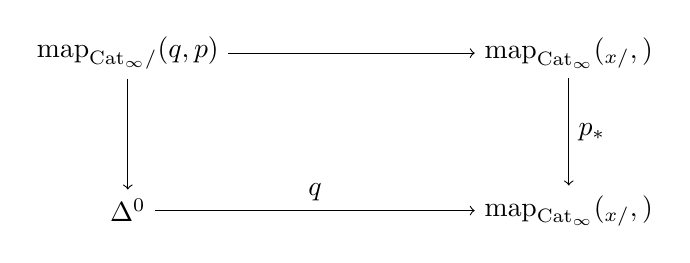
\begin{tikzpicture}
  \node (mp) at (0,0) {$\mathrm{map}_{\mathrm{Cat}_{\infty}/\C}(q, p)$};
  \node (mc) at (5.6,0) {$\mathrm{map}_{\mathrm{Cat}_{\infty}}(\C_{x/}, \E)$};
  \node (d0) at (0,-2.0) {$\Delta^0$};
  \node (mq) at (5.6,-2.0) {$\mathrm{map}_{\mathrm{Cat}_{\infty}}(\C_{x/}, \C)$};
  \draw[->] (mp) -- (mc);
  \draw[->] (mp) -- (d0);
  \draw[->] (mc) -- node[right] {$p_*$} (mq);
  \draw[->] (d0) -- node[above] {$q$} (mq);
\end{tikzpicture}
\end{center}
我们现在回忆一下，由第 2 章中的\cref{thm:coherent-nerve-mapping-space}，
$\mathrm{Cat}_{\infty}$ 中的诸\trMappingSpace{}典范地等价于\trFunctor{}范畴的%
\trGroupoid{}核。
于是，上述图表中右边的竖直映射与下述图表中左边的竖直映射等同：
\begin{center}
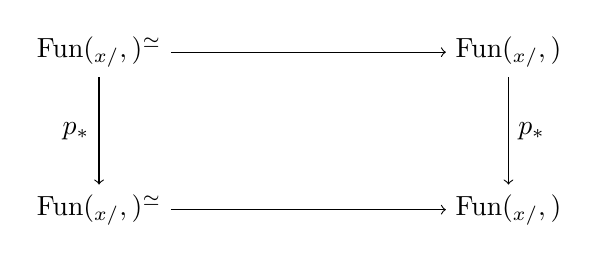
\begin{tikzpicture}
  \node (fe) at (0,0) {$\mathrm{Fun}(\C_{x/}, \E)^{\simeq}$};
  \node (fx) at (5.2,0) {$\mathrm{Fun}(\C_{x/}, \E)$};
  \node (fc) at (0,-2.0) {$\mathrm{Fun}(\C_{x/}, \C)^{\simeq}$};
  \node (fq) at (5.2,-2.0) {$\mathrm{Fun}(\C_{x/}, \C)$};
  \draw[->] (fe) -- (fx);
  \draw[->] (fe) -- node[left] {$p_*$} (fc);
  \draw[->] (fx) -- node[right] {$p_*$} (fq);
  \draw[->] (fc) -- (fq);
\end{tikzpicture}
\end{center}
由于 $p$ 是一个\trLeftFibration{}，由第 1 章中的\cref{thm:angle-fi-fibration}，
$p_*$ 也是一个\trLeftFibration{}。\footnote{译注：原书印作「right fibration」，与
p.215「$p\colon \E \to \C$ be the left fibration」相抵；据定理 1.3.37(1)（取
$A=\varnothing$）知 $p^*$ 与 $p$ 同手性，结论不受影响，此处径改。——译者注}于是，
由第 2 章中的%
\cref{prop:left-right-fibrations-conservative}，映射 $p_*$ 是\trConservative{}，
从而由\cref{ex:conservative-pullback}，该图表是一个\trPullback{}。把这两个图表拼接起来，我们发现方块
\begin{center}
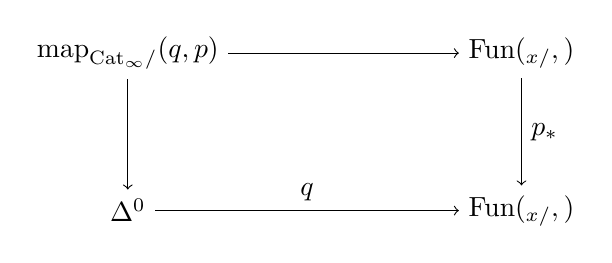
\begin{tikzpicture}
  \node (mp) at (0,0) {$\mathrm{map}_{\mathrm{Cat}_{\infty}/\C}(q, p)$};
  \node (fe) at (5.0,0) {$\mathrm{Fun}(\C_{x/}, \E)$};
  \node (d0) at (0,-2.0) {$\Delta^0$};
  \node (fq) at (5.0,-2.0) {$\mathrm{Fun}(\C_{x/}, \C)$};
  \draw[->] (mp) -- (fe);
  \draw[->] (mp) -- (d0);
  \draw[->] (fe) -- node[right] {$p_*$} (fq);
  \draw[->] (d0) -- node[above] {$q$} (fq);
\end{tikzpicture}
\end{center}
是\trHomotopyCartesian{}。由于 $\mathrm{Fun}_q(\C_{x/}, \E)$ 是这个图表的%
\trPullback{}，我们发现典范映射
\[
\mathrm{map}_{\mathrm{Cat}_{\infty}/\C}(q, p) \to \mathrm{Fun}_q(\C_{x/}, \E)
\]
如所断言是一个\trJoyalEquivalence{}。
\end{proof}

借助于这个结果，我们几乎得到了\trYoneda{}引理通常的推论，即\trYoneda{}\trFunctor{}是%
\trFullyFaithful{}。从现在起，它将被称为\emph{\trYoneda{}嵌入}。

\begin{proposition}\label{prop:yoneda-embedding}
设 $\C$ 是一个∞-\trCategory{}。那么\trYoneda{}\trFunctor{}%
$Y\colon \C \to \mathrm{Fun}(\C^{\mathrm{op}}, \mathrm{Spc})$
是\trFullyFaithful{}。
\end{proposition}

\begin{proof}
我们只需计算：求值映射
\[
\mathrm{map}_{\mathrm{Fun}(\C^{\mathrm{op}}, \mathrm{Spc})}
  \bigl(\mathrm{map}_{\C}(-, x), \mathrm{map}_{\C}(-, y)\bigr)
  \longrightarrow \mathrm{map}_{\C}(x, y)
\]
由\cref{prop:yoneda-lemma}是一个\trEquivalence{}，并断言复合
\[
\mathrm{map}_{\C}(x, y) \xrightarrow{\;Y\;}
  \mathrm{map}_{\mathrm{Fun}(\C^{\mathrm{op}}, \mathrm{Spc})}
  \bigl(\mathrm{map}_{\C}(-, x), \mathrm{map}_{\C}(-, y)\bigr)
  \longrightarrow \mathrm{map}_{\C}(x, y)
\]
也是一个\trEquivalence{}。非形式地说，它显然就是恒同，但一个形式化的证明需要更多的功夫，
这正是我们不在这里把它做出来的原因。（更多的解释见下述评注。）总而言之，我们
得到：\trYoneda{}\trFunctor{}在诸\trMappingSpace{}上诱导出一个等价，这就证明了本命题。
\end{proof}

\begin{remark}\label{rem:hebestreit-yoneda}
定义\trBivariant{}\trMappingSpace{}\trFunctor{}的另一种方式由\trHebestreit{}（Fabian Hebestreit）向我们建议：
我们可以把源--目标\trFunctor{} $\mathrm{Fun}(\Delta^1, \C) \to \C \times \C$ 视为
$\C$ 之上的一个\trFunctor{}，其做法是经由源映射与到第一因子的投射，而这两者都是%
\trCartesianFibration{}。此外，源--目标映射保持笛卡尔\trMorphism{}，于是该图表
提供一个映射
\[
\Delta^1 \longrightarrow \mathrm{Cart}(\C)
  \simeq \mathrm{Fun}(\C^{\mathrm{op}}, \mathrm{Cat}_\infty).
\]
作伴随，我们便得到一个\trFunctor{}%
\[
\C^{\mathrm{op}} \longrightarrow \mathrm{Fun}(\Delta^1, \mathrm{Cat}_\infty)
\]
它——把诸定义展开来看——把 $x$ 送到投射\trFunctor{} $\C_{x/} \to \C$。由于这是一个%
\trLeftFibration{}，而\trLeftFibration{}又是
$\mathrm{Fun}(\Delta^1, \mathrm{Cat}_\infty)$ 的一个满子\trCategory{}，
我们便得到一个\trFunctor{}%
\[
\C^{\mathrm{op}} \longrightarrow \mathrm{LFib}(\C)
  \simeq \mathrm{Fun}(\C, \mathrm{Spc}),
\]
它是\trYoneda{}\trFunctor{}的另一个候选者，因为它把 $x$ 送到表示\trFunctor{}%
$\mathrm{map}_{\C}(x, -)$ 的那个\trLeftFibration{} $\C_{x/} \to \C$。这一做法的
优点是：可以从定义出发证明这个\trYoneda{}\trFunctor{}%
$\C^{\mathrm{op}} \to \mathrm{Fun}(\C, \mathrm{Spc})$ 是\trFullyFaithful{}，
见\trHebestreit{}的讲义
\cite[Yoneda's lemma, adjunctions, and (co)limits]{Heb20}。遗憾的是，下述两条陈述都不显然：
\begin{enumerate}[label=(\arabic*)]
  \item 如上构造的\trFunctor{} $\C^{\mathrm{op}} \times \C \to \mathrm{Spc}$ 等价于%
        \cref{def:yoneda-functor}中经\trTwistedArrowCategory{}构造的那一个。
  \item 如上构造的\trFunctor{} $\C^{\mathrm{op}} \times \C \to \mathrm{Spc}$ 等价于其对偶
        版本，在后一版本中，我们利用靶映射与到第二因子的投射，把源--目标映射视为
        诸\trCocartesianFibration{}之间的一个映射。
\end{enumerate}
结果表明，这两条陈述都成立，但它们的证明需要更多的工具。
\end{remark}
